\documentclass[twocolumn,aps,american,pra,nofootinbib,superscriptaddress,longbibliography,floatfix]{revtex4-2}
\usepackage{graphicx,graphics,epsfig,subfigure,times,bm,bbm,amssymb,amsmath,amsfonts,amsthm,mathrsfs,MnSymbol,accents}
\usepackage[pdftex]{color}
\usepackage{tikz}

\begin{document}

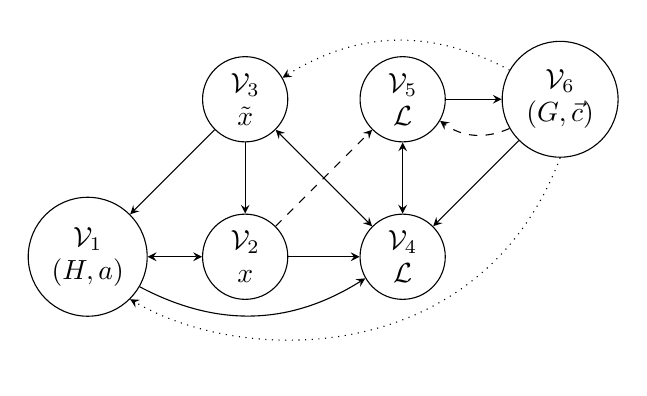
\begin{tikzpicture}
  \newlength{\dx}
  \newlength{\dy}
  \setlength{\dx}{2cm}
  \setlength{\dy}{2cm}
  \node[draw,circle,align=center](n1) at (-2\dx, 0)
    {$\mathcal{V}_1$\\$(H,a)$};
  \node[draw,circle,align=center](n2) at (-1\dx, 0)
    {$\mathcal{V}_2$\\$x$};
  \node[draw,circle,align=center](n3) at (-\dx,\dy)
    {$\mathcal{V}_3$\\$\tilde{x}$};
  \node[draw,circle,align=center](n4) at (    0, 0)
    {$\mathcal{V}_4$\\$\mathcal{L}$};
  \node[draw,circle,align=center](n5) at (   0,\dy)
    {$\mathcal{V}_5$\\$\mathcal{L}$};
  \node[draw,circle,align=center](n6) at ( \dx,\dy)
    {$\mathcal{V}_6$\\$(G,\vec{c})$};
  \draw[stealth-stealth] (n1) -- (n2);
  \draw[stealth-stealth] (n3) -- (n4);
  \draw[stealth-stealth] (n4) -- (n5);
  \draw[-stealth] (n3) -- (n1);
  \draw[-stealth] (n3) -- (n2);
  \draw[-stealth] (n2) -- (n4);
  \draw[-stealth] (n5) -- (n6);
  \draw[-stealth] (n6) -- (n4);
  \path[-stealth] (n1) edge[bend right] (n4);
  \path[dashed,-stealth] (n6) edge[bend left] (n5);
  \draw[dashed,-stealth] (n2) -- (n5);
  \path[dotted,-stealth] (n6) edge[bend right] (n3);
  \draw[dotted,-stealth] (n6.south)
    ..controls (0.5\dx,-0.7\dy) and (-\dx,-0.7\dy).. (n1.south east);
\end{tikzpicture}

\end{document}